\section{Stochastic Blockmodels}\label{sec:SBMs}

Describe generic algorithm without specifying if its the party/topic model

\subsection{Artificial Neural Network Adaptation}\label{sec:ANNAdaptation}

\subsubsection{Stochastic Party Leader Blockmodel}\label{sec:SPLBM}

The stochastic party leader model generates user behaviour only taking into
account the previous party leaders each user had engaged with prior. For each
user, when deciding which tweet they are to retweet, their retweet history is
converted into a probability distribution (ex.\
$history=[JT=0,AS=1,JS=3,EM=2,MB=0]$ generates
$probs=[JT=0.09,AS=0.19,JS=0.36,EM=0.27,MB=0.09]$). In this sense, it models a
world in which politically engaged Twitter users only engage along the axis of
party leaders, with a complete disregard for the topics tweeted about. Figure
\ref{fig:stochastic_party_leader_model} shows two examples of stochastic party
leader blockmodels: one in which edge probabilities are proportional the number
of times that user's retweeted each party leader, and one in which edge
probabilities are determined with the ANN described in section
\ref{sec:ANNAdaptation}.

\begin{singlespacing}
    \begin{figure}
        \centering
        \begin{tabular}{cc}
          \includegraphics[width=50mm]{Figures/simple_stochastic_party_leader_model}
          &
          \includegraphics[width=50mm]{Figures/ann_stochastic_party_leader_model}
          \\
        (a) Simple Stochastic Party Leader Blockmodel & (b) ANN Adaption\\[6pt]
        \end{tabular}
        \caption[Stochastic Party Leader Blockmodels]{Stochastic Party Leader Blockmodels}
        \label{fig:stochastic_party_leader_model}
    \end{figure}
\end{singlespacing}

\subsubsection{Stochastic Topic Blockmodel}\label{sec:STBM}

Conversely, the stochastic topic blockmodel models a world in which politically
engaged Twitter users only engage along the axis of topics. Here, the topic
history of a user is converted into a probability distribution, and with a
probability of $\epsilon$, that user will retweet the topic with the highest
activation -- regardless of which party leader tweeted it. Figure
\ref{fig:stochastic_topic_model} shows two examples of stochastic topic
blockmodels: in which edge probabilities are proportional to a user's topic
retweet history, and one in which edge probabilities are determined with the ANN
described in section \ref{sec:ANNAdaptation}.

\begin{singlespacing}
    \begin{figure}
        \centering
        \begin{tabular}{cc}
          \includegraphics[width=50mm]{Figures/simple_stochastic_topic_model} &
          \includegraphics[width=50mm]{Figures/ann_stochastic_topic_model} \\
        (a) Simple Stochastic Topic Blockmodel & (b) ANN Adaption\\[6pt]
        \end{tabular}
        \caption[Stochastic Topic Blockmodels]{Stochastic Topic Blockmodels}
        \label{fig:stochastic_topic_model}
    \end{figure}
\end{singlespacing}

\subsubsection{Stochastic Hybrid Blockmodel}\label{sec:SHBM}

The final model developed is a hybrid of the stochastic party leader block
model, and the stochastic topic blockmodel. Here, two history vectors for each
user are captured -- the $n$ dimensional party leader history vector, and the
$k$ dimensional topic history vector. After each respective vector is converted
into a probability distribution, the weight of a retweet of topic $i$ by party
leader $j$ is determined by some constant $\alpha$\footnote{This has no relation
to the parameter $\alpha$ referred to in section \ref{sec:LDA}} and the
function:

\begin{equation}
    weight(party leader=i, topic=j)=\alpha P(i)+(1-\alpha)P(j)
\end{equation}

Where $P(i)$ is index $i$ of that user's \emph{party leader} probability
distribution, $P(j)$ is index $j$ of that user's \emph{topic} probability
distribution, and $\alpha$ is some constant that determines the relative
weighting of the two. As $\alpha$ approaches $1$, the hybrid model becomes
equivalent to the stochastic party leader blockmodel -- and as $\alpha$
approaches $0$ the model approaches the stochastic topic blockmodel. This model
then generates different ``worlds'' in which users' political engagement falls
on the spectrum from only caring about \emph{party leaders} to only caring about
\emph{topics}.

\subsection{NetLSD for Describing Political Engagement}\label{sec:NetLSDForSBM}

The final objective of comparing the relative importance of topics and party
leaders in driving political engagement requires comparing the structure of
target graph shown in \ref{ch:GraphTheory}, and various hybrid models generated
with different values of $\alpha$. Using the Network Laplacian Spectral
Descriptor described in section \ref{sec:NetLSD} by Tsitsulin et al. the optimal
alpha value can be determined in a scale-adaptive, size-invariant, and
permutation-invariant manner \cite{netlsd}.

Given the $O(n^{3})$ complexity involved in calculating the eigenvalues of a
graphs normalized Laplacian matrix it is advantageous to generate sufficiently
small hybrid models when fitting them to the original engagement graph (see
figure \ref{fig:og_graph}). To determine how large a graph of this nature needs
to be to capture its underlying structure -- tweets of the original graph were
sampled, keeping all the retweet edges, and then compared to the heat trace
signature of the original graph. This is shown graphically in figure
\ref{fig:dist_from_original_graph_over_sample_size}, the x-axis represents how
many tweets \emph{per party leader} were sampled from the original graph and the
y-axis represents the $L_{2}$ distance from the original engagement graph's heat
trace signature. 

\begin{singlespacing}
    \begin{figure}[H]
    \centering
    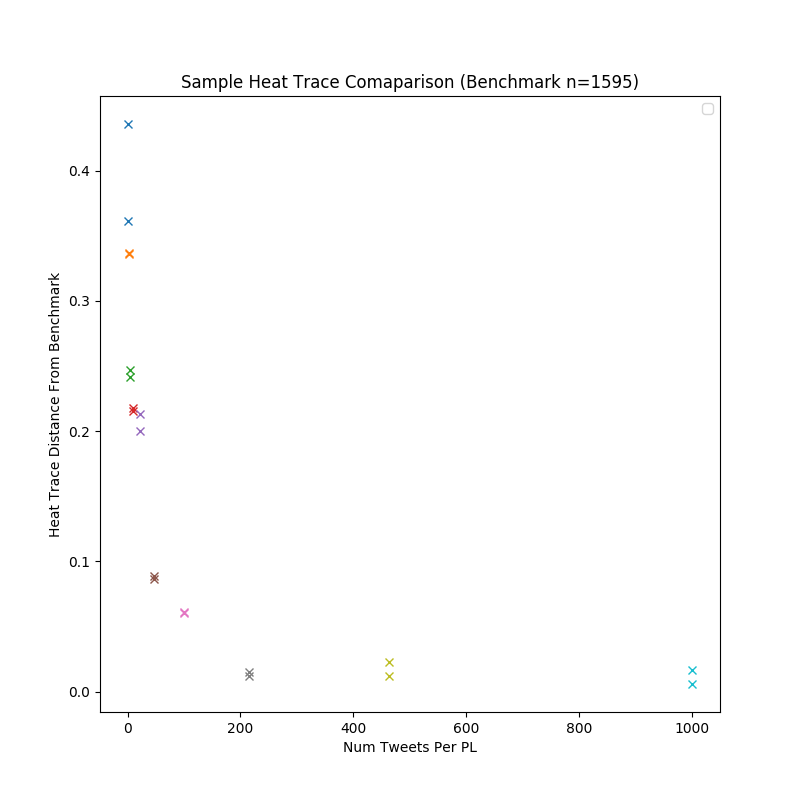
\includegraphics[scale=0.4]{Figures/dist_from_original_graph_over_sample_size}
    \caption[Heat Trace Signature Distance as a Function of Graph Sample Size]{Heat Trace Signature Distance as a Function of Graph Sample Size}
    \label{fig:dist_from_original_graph_over_sample_size}
    \end{figure}
\end{singlespacing}

As can be seen from figure \ref{fig:dist_from_original_graph_over_sample_size}, there
are diminishing returns for graphs with more than 215 tweets per party leader.
Therefore, for each of the party leader vertices generated with the hybrid
models -- each one generated a number of tweets by a random variable $X$ that is
distributed normally where $X \sim \mathcal{N}(\mu=215,\,\sigma^{2}=70)$.

\subsection{Results}\label{sec:SBMsResults}

